%!TEX root = main.tex
\def\mypolygonscale{0.9}
\def\myyscale{1.2}
\def\myxscale{1.0}
\definecolor{mygreen}{cmyk}{0.5,0,0.5,0.5}
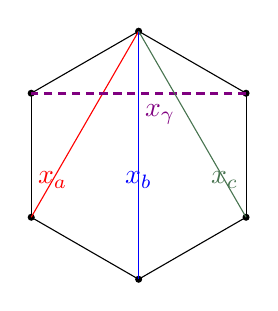
\begin{tikzpicture}[scale = \mypolygonscale]
%\tikzstyle{every node} = [font = \small]
\foreach \x in {0}
{
    \foreach \y in {-8}
    {
			\fill (\x,\y+1.75) circle (.05);
			%\fill (\x,\y+1.75) node [above] {\tiny{$1$}};
			\fill(\x+1.5158,\y+.875) circle (.05);
			%\fill (\x+1.5158,\y+.875) node [right] {\tiny{$2 $}};
			\fill (\x+1.5158,\y-.875) circle (.05);
			%\fill (\x+1.5158,\y-.875) node [right] {\tiny{$3$}};
			\fill(\x,\y-1.75) circle (.05);
			%\fill (\x,\y-1.75) node [below] {\tiny{$4$}};
			\fill(\x-1.5158,\y-.875) circle (.05);
			%\fill (\x-1.5158,\y-.875) node [left] {\tiny{$5$}};
			\fill (\x-1.5158,\y+.875) circle (.05);
			%\fill (\x-1.5158,\y+.875) node [left] {\tiny{$6$}};
		
			\draw [] (\x,\y+1.75)--(\x+1.5158,\y+.875); %v1 to v2
			\draw [] (\x+1.5158,\y+.875) -- (\x+1.5158,\y-.875); %v3 to v2
			\draw [] (\x+1.5158,\y-.875)--(\x,\y-1.75); %v4 to v3
			\draw [] (\x,\y-1.75) -- (\x-1.5158,\y-.875); %v5 to v4
			\draw [] (\x-1.5158,\y-.875)--(\x-1.5158,\y+.875); %v6 to v5
			\draw [] (\x-1.5158,\y+.875) -- (\x,\y+1.75); %v1 to v6
		
\draw [red] (\x,\y+1.75) -- (\x-1.5158,\y-.875) node[pos=0.8] {$x_a$};
%\draw[->,densely dotted, thick]  (\x,\y) -- (\x-1.5158*0.5,\y + 1.75*.5 - .875*.5); 
%\draw ((\x+\x-1.5158)*0.5,(\y+\y1.75 - .875)*.5) -- (\x,\y+1.75); 
\draw [blue] (\x,\y+1.75) -- (\x,\y-1.75) node[pos=0.6] {$x_b$};
%\draw[densely dashed, ultra thick,rounded corners=2mm]  (\x+1.5158,\y+.875) -- (\x+1.5158*0.5,\y + 1.75*.5 - .875*.5) -- (\x,\y) --  (\x-1.5158*0.5,\y + 1.75*.5 - .875*.5) -- (\x-1.5158,\y+.875); 
\draw[densely dashed, very thick, violet]  (\x+1.5158,\y+.875)  -- (\x-1.5158,\y+.875) node[pos=0.4,below] {$x_\gamma$}; 
\draw [mygreen] (\x,\y+1.75) -- (\x+1.5158,\y-.875) node[pos=0.8] {$x_c$};
	}
} 
\end{tikzpicture}% end gamma 
\quad\quad
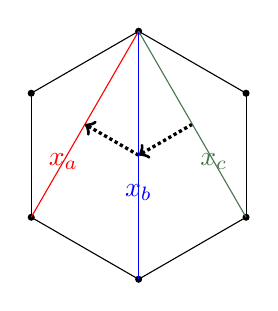
\begin{tikzpicture}[scale = \mypolygonscale]
%\tikzstyle{every node} = [font = \small]
\foreach \x in {0}
{
    \foreach \y in {-8}
    {
			\fill (\x,\y+1.75) circle (.05);
			%\fill (\x,\y+1.75) node [above] {\tiny{$1$}};
			\fill(\x+1.5158,\y+.875) circle (.05);
			%\fill (\x+1.5158,\y+.875) node [right] {\tiny{$2 $}};
			\fill (\x+1.5158,\y-.875) circle (.05);
			%\fill (\x+1.5158,\y-.875) node [right] {\tiny{$3$}};
			\fill(\x,\y-1.75) circle (.05);
			%\fill (\x,\y-1.75) node [below] {\tiny{$4$}};
			\fill(\x-1.5158,\y-.875) circle (.05);
			%\fill (\x-1.5158,\y-.875) node [left] {\tiny{$5$}};
			\fill (\x-1.5158,\y+.875) circle (.05);
			%\fill (\x-1.5158,\y+.875) node [left] {\tiny{$6$}};
		
			\draw [] (\x,\y+1.75)--(\x+1.5158,\y+.875); %v1 to v2
			\draw [] (\x+1.5158,\y+.875) -- (\x+1.5158,\y-.875); %v3 to v2
			\draw [] (\x+1.5158,\y-.875)--(\x,\y-1.75); %v4 to v3
			\draw [] (\x,\y-1.75) -- (\x-1.5158,\y-.875); %v5 to v4
			\draw [] (\x-1.5158,\y-.875)--(\x-1.5158,\y+.875); %v6 to v5
			\draw [] (\x-1.5158,\y+.875) -- (\x,\y+1.75); %v1 to v6
		
\draw [red] (\x,\y+1.75) -- (\x-1.5158,\y-.875) node[pos=0.7] {$x_a$};
\draw[->,densely dotted, very thick] (\x,\y) -- (\x-1.5158*0.5,\y + 1.75*.5 - .875*.5); 
%\draw ((\x+\x-1.5158)*0.5,(\y+\y1.75 - .875)*.5) -- (\x,\y+1.75); 
\draw [blue] (\x,\y+1.75) -- (\x,\y-1.75) node[pos=0.65] {$x_b$};
\draw[->,densely dotted, very thick]  (\x+1.5158*0.5,\y + 1.75*.5 - .875*.5) -- (\x,\y); 
\draw [mygreen] (\x,\y+1.75) -- (\x+1.5158,\y-.875) node[pos=0.7] {$x_c$};
	}
}
\end{tikzpicture}
\quad\quad
Let $Q_\gamma=$
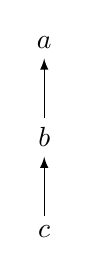
\begin{tikzpicture}[yscale=\myyscale, xscale=\myxscale, line join=bevel,
>=latex, 
%font = \small
]
\def\posetedgecolor{blue}
\node(c) at (0,0) {{$c$}}; %{$1$};
\node(b) at (0,1) {{$b$}}; %{$2$};
\node(a) at (0,2) {{$a$}}; %{$3$};

\draw[->] (c) -- (b) ;%node[\posetedgecolor,pos=0.5] {$0$}; 
\draw[->] (b) -- (a) ;%node[\posetedgecolor,pos=0.5] {$1$}; 
\end{tikzpicture}